\documentclass[conference]{IEEEtran}
\IEEEoverridecommandlockouts

\usepackage{cite}
\usepackage{amsmath,amssymb,amsfonts}
\usepackage{algorithmic}
\usepackage{graphicx}
\usepackage{textcomp}
\usepackage{xcolor}
\usepackage{booktabs}
\usepackage{multirow}
\usepackage{subcaption}
\usepackage{hyperref}
\usepackage{array}
\usepackage{balance}

\def\BibTeX{{\rm B\kern-.05em{\sc i\kern-.025em b}\kern-.08em
    T\kern-.1667em\lower.7ex\hbox{E}\kern-.125emX}}

\begin{document}

\title{Deep Convolutional Neural Networks for Fine-Grained Spice Image Classification}

\author{
\IEEEauthorblockN{Noushad}
\IEEEauthorblockA{
\textit{SpiceNet Research}\\
noushad@spicenet.ai}
}

\maketitle

% ─────────────────────────────────────────────────────────────────────────────
\begin{abstract}
Accurate automated spice identification poses a significant challenge in computer
vision due to high visual similarity across spice categories, overlapping color
distributions, and near-identical texture patterns—especially in powdered or ground
form. Existing food recognition systems either exclude spices entirely or treat them
as coarse-level categories, limiting practical applicability. We present
\textbf{SpiceFusionNet}, a multi-modal deep learning framework that jointly exploits
three complementary representations: (1) a pretrained EfficientNet-B4 backbone for
global feature extraction, (2) a texture branch combining Local Binary Pattern (LBP)
and Gray-Level Co-occurrence Matrix (GLCM) descriptors fed through a shallow MLP,
and (3) a color branch encoding HSV histograms with spice-calibrated bins. The three
branches are merged via learned attention-weighted late fusion. Training proceeds in
three phases: supervised backbone pre-training, Supervised Contrastive (SupCon)
fine-tuning on hard-negative spice pairs, and end-to-end fusion training. Evaluated
on \textit{SpiceSpectrum}—a class-balanced dataset of 11,000 images across 11
commercially valuable spice cultivars—our method achieves \textbf{99.00\%} Top-1
accuracy and \textbf{99.95\%} Top-5 accuracy at \textbf{2.70\,ms} per image,
dramatically outperforming traditional SVM with HOG and color histogram features
(32.49\%) and remaining competitive with strong deep-learning baselines. Grad-CAM
visualizations confirm that the model attends to discriminative spice texture and
color regions rather than background artifacts. The work has direct implications for
smart kitchen assistants, food quality control, and retail spice inventory management.
\end{abstract}

\begin{IEEEkeywords}
fine-grained visual recognition, spice classification, multi-modal fusion,
contrastive learning, EfficientNet, texture features, food recognition
\end{IEEEkeywords}


% ─────────────────────────────────────────────────────────────────────────────
\section{Introduction}
\label{sec:intro}

Spices constitute an essential ingredient of culinary traditions across the globe,
representing a market valued at over USD~20 billion annually~\cite{spicemarket2023}.
Despite their economic importance, automated visual identification of spices remains
underexplored in the computer vision literature. The core difficulty lies in
fine-grained inter-class similarity: cumin and coriander seeds appear almost
identical under standard imaging conditions; turmeric and paprika powders share
nearly the same orange-yellow hue; cloves and black pepper are both small, dark, and
spheroidal. Even trained human observers make errors when samples are presented
without contextual packaging.

Current food recognition benchmarks—Food-101~\cite{bossard14}, UEC-Food256, and
related datasets—either omit spices entirely or reduce them to coarse categories
(e.g., ``seasoning''), leaving a significant research gap. At the same time, the
growing penetration of smart kitchen devices and AI-assisted food safety systems
creates clear industrial demand for precise, real-time spice recognition.

In this work we address the gap by:
\begin{enumerate}
    \item Designing \textbf{SpiceFusionNet}, a multi-modal CNN that fuses global CNN
          features with explicit texture and color representations extracted by
          classical image descriptors.
    \item Proposing a \textbf{three-phase training curriculum} that combines
          cross-entropy pre-training with Supervised Contrastive Learning (SupCon)
          fine-tuning on visually confusable spice pairs.
    \item Conducting comprehensive experiments on the \textit{SpiceSpectrum}
          dataset~\cite{spicespectrum2025} against four baselines
          (ResNet-50, EfficientNet-B4, ViT-Base, SVM) and five backbone variants.
    \item Providing interpretability through Grad-CAM~\cite{selvaraju2017grad}
          saliency maps.
\end{enumerate}

Our results demonstrate that SpiceFusionNet achieves 99.00\% Top-1 accuracy—a
dramatic improvement over the SVM baseline (32.49\%)—while maintaining real-time
inference at 2.70\,ms per image on a consumer GPU.


% ─────────────────────────────────────────────────────────────────────────────
\section{Related Work}
\label{sec:related}

\subsection{Food and Ingredient Recognition}
Bossard et al.~\cite{bossard14} introduced Food-101 and demonstrated that CNN
features transfer well to fine-grained food classification. He et al.~\cite{he2016deep}
showed that deep residual networks significantly improved general image recognition.
More recent transformer-based models~\cite{dosovitskiy2020image} further advance
state-of-the-art on fine-grained benchmarks. However, none of these works
specifically address the challenges of spice recognition.

\subsection{Fine-Grained Visual Recognition}
Fine-grained visual recognition (FGVR) aims to distinguish subcategories within a
superclass. Bilinear pooling~\cite{lin2015bilinear}, part-based attention, and
contrastive feature learning have all been applied to FGVR. Our approach borrows
from this tradition by adding explicit texture/color branches to capture the
discriminative micro-texture and color palette that characterize different spices.

\subsection{Multi-Modal Feature Fusion}
Combining deep CNN features with handcrafted descriptors has been explored for
texture classification~\cite{cimpoi2014describing}. LBP~\cite{ojala2002multiresolution}
and GLCM~\cite{haralick1973textural} remain competitive low-dimensional texture
descriptors. We integrate these classical features into a modern deep fusion
architecture via learned attention weighting.

\subsection{Contrastive Learning}
Supervised Contrastive Learning (SupCon)~\cite{khosla2020supervised} extends
self-supervised contrastive objectives to fully supervised settings by using labels
to define positive pairs. We apply SupCon in Phase~2 specifically targeting visually
confusable spice pairs (e.g., cumin/coriander, paprika/turmeric), improving feature
discriminability before the fusion head is introduced.


% ─────────────────────────────────────────────────────────────────────────────
\section{Dataset}
\label{sec:dataset}

We use the \textit{SpiceSpectrum}~\cite{spicespectrum2025} dataset, a publicly
available class-balanced collection of 11,000 high-resolution images covering
11 commercially valuable spice cultivars: black pepper, cardamom, cinnamon, cloves,
coriander, cumin, ginger, nutmeg, paprika, saffron, and turmeric.
Each class contains exactly 1,000 images at 512$\times$512 pixel resolution
acquired under diverse lighting conditions, backgrounds, and presentation forms
(whole, ground, and dried), collected from open-source repositories
(Open Images, iNaturalist) and self-captured macro-photography.

\subsection{Data Splits}
Following the paper's protocol, we apply stratified splitting:
\textbf{70\%} train (7,700 images),
\textbf{10\%} validation (1,100 images), and
\textbf{20\%} test (2,200 images), ensuring all presentation forms appear in every
split.

\subsection{Preprocessing and Augmentation}
Input images are resized to 224$\times$224 for model input and normalized with
ImageNet statistics ($\mu = [0.485, 0.456, 0.406]$,
$\sigma = [0.229, 0.224, 0.225]$). Spice-specific augmentation
is applied during training:
\textit{RandomResizedCrop} (scale 0.7–1.0), horizontal/vertical flips,
rotation ($\pm 30°$), \textit{ColorJitter} (brightness, contrast, saturation 0.3;
hue 0.1), Gaussian/motion blur, Gaussian noise, and CoarseDropout.
Validation and test images are processed only with center-crop normalization.

Hand-crafted features (LBP, GLCM, HSV) are extracted from the \emph{original}
512$\times$512 image before augmentation, providing a stable signal that is
consistent between training and inference.

\subsection{SAM-Augmented Variant}
To study the effect of background clutter, we additionally create a
\textit{SpiceSpectrum-SAM} variant by applying Meta's Segment Anything Model
(SAM)~\cite{kirillov2023segment} via center-point prompts to isolate spice regions
from their backgrounds (white fill). This allows direct comparison of raw vs.
segmentation-preprocessed training data.


% ─────────────────────────────────────────────────────────────────────────────
\section{Methodology}
\label{sec:method}

\subsection{SpiceFusionNet Architecture}

SpiceFusionNet processes each input through three parallel branches whose outputs
are combined by a learned attention fusion module, followed by a classification
head. Figure~\ref{fig:arch} illustrates the overall architecture.

\subsubsection{CNN Branch}
We adopt EfficientNet-B4~\cite{tan2019efficientnet} pretrained on ImageNet-1k as
the backbone. With the classification head removed, the backbone outputs a
1,792-dimensional global average-pooled feature vector $\mathbf{f}_{\text{cnn}}$.

\subsubsection{Texture Branch}
For each image we extract:
\begin{itemize}
    \item \textbf{LBP histogram:} Uniform LBP with $P=8$ neighbors and radius $R=1$
          produces a 10-dimensional normalized histogram over the grayscale image.
    \item \textbf{GLCM features:} Gray-level co-occurrence matrices computed at
          distances $\{1, 2\}$ and angles $\{0°, 45°, 90°, 135°\}$ (64 gray levels)
          yield six properties (contrast, dissimilarity, homogeneity, energy,
          correlation, ASM) $\times$ 8 distance-angle combinations = 48 values.
\end{itemize}
The resulting 58-dimensional texture vector is processed by a two-layer MLP
(58 $\to$ 128 $\to$ 256) with BatchNorm, ReLU, and dropout to produce
$\mathbf{f}_{\text{tex}} \in \mathbb{R}^{256}$.

\subsubsection{Color Branch}
HSV color histograms are computed with spice-calibrated bins
(H: 36, S: 32, V: 32 bins), producing a 100-dimensional vector. A two-layer MLP
(100 $\to$ 64 $\to$ 128) outputs $\mathbf{f}_{\text{col}} \in \mathbb{R}^{128}$.

\subsubsection{Attention Fusion}
The concatenated representation
$\mathbf{f} = [\mathbf{f}_{\text{cnn}}, \mathbf{f}_{\text{tex}}, \mathbf{f}_{\text{col}}]$
is passed through a linear gate:
\begin{equation}
    \mathbf{g} = \text{softmax}(W\mathbf{f} + b), \quad \mathbf{g} \in \mathbb{R}^3
    \label{eq:gate}
\end{equation}
The gated output $\tilde{\mathbf{f}} = [g_1\mathbf{f}_{\text{cnn}},\,
g_2\mathbf{f}_{\text{tex}},\, g_3\mathbf{f}_{\text{col}}]$ is fed to the
classification head: FC(2176 $\to$ 512) $\to$ BN $\to$ ReLU $\to$ Dropout(0.4)
$\to$ FC(512 $\to$ 11).

\subsection{Three-Phase Training Strategy}

\subsubsection{Phase 1 — Supervised Pre-training}
The EfficientNet-B4 backbone and an image-only classification head are fine-tuned
with cross-entropy loss (label smoothing $\epsilon=0.1$), AdamW
($\text{lr}=10^{-4}$, $\lambda=10^{-4}$), and a cosine learning-rate schedule
with 3-epoch linear warmup, for up to 30 epochs with early stopping
(patience = 8). This yields a strong unimodal baseline before fusion.

\subsubsection{Phase 2 — Contrastive Fine-tuning}
With the backbone loaded from Phase~1, we freeze all parameters except the backbone
and a projection head (1792 $\to$ 512 $\to$ 128). We apply the Supervised
Contrastive loss~\cite{khosla2020supervised}:
\begin{equation}
    \mathcal{L}_{\text{SupCon}} = \sum_{i} \frac{-1}{|P(i)|} \sum_{p \in P(i)}
    \log \frac{e^{\mathbf{z}_i \cdot \mathbf{z}_p / \tau}}
    {\sum_{a \neq i} e^{\mathbf{z}_i \cdot \mathbf{z}_a / \tau}}
    \label{eq:supcon}
\end{equation}
where $\tau = 0.07$, $\mathbf{z}$ are $\ell_2$-normalized projection features, and
$P(i)$ is the set of same-class samples in the batch. This phase runs for
10 epochs with $\text{lr}=5 \times 10^{-5}$, specifically improving discrimination
among hard-negative pairs (cumin/coriander, paprika/turmeric, black pepper/cloves,
cinnamon/nutmeg).

\subsubsection{Phase 3 — Full Fusion End-to-end Training}
All branches and the fusion head are trained jointly for 10 epochs
($\text{lr}=10^{-5}$, cosine decay) using a combined loss:
\begin{equation}
    \mathcal{L} = \alpha\,\mathcal{L}_{\text{CE}} + (1-\alpha)\,\mathcal{L}_{\text{SupCon}},
    \quad \alpha = 0.5
    \label{eq:combined}
\end{equation}
Gradient clipping at 1.0 is applied throughout all phases.


% ─────────────────────────────────────────────────────────────────────────────
\section{Experiments}
\label{sec:experiments}

\subsection{Implementation Details}
All experiments use PyTorch 2.11.0 on an NVIDIA GeForce RTX 5060 Ti (16 GB VRAM).
The batch size is 32 for all phases. Data loading uses 4 worker processes. ImageNet
pretrained weights are loaded via \texttt{timm}~\cite{rw2019timm}. Albumentations
2.0.8~\cite{info11020125} is used for augmentation. scikit-learn 1.4.0 provides
the SVM and metric utilities. All experiments are seeded with seed 42 for
reproducibility.

\subsection{Evaluation Protocol}
We report Top-1 accuracy, Top-5 accuracy, macro-averaged F1-score, weighted
F1-score, per-class precision/recall/F1, and inference latency (ms/image,
averaged over 20 batches on GPU).

\subsection{Baselines}
Four baselines are evaluated under identical data splits and augmentation:
\begin{enumerate}
    \item \textbf{SVM} with HOG (26,244-d) + HSV histogram (100-d) features,
          LinearSVC with PCA(256) dimensionality reduction.
    \item \textbf{ResNet-50}~\cite{he2016deep} fine-tuned end-to-end.
    \item \textbf{EfficientNet-B4}~\cite{tan2019efficientnet} fine-tuned
          (image-only, no fusion modules).
    \item \textbf{ViT-Base/16}~\cite{dosovitskiy2020image} fine-tuned.
\end{enumerate}
All deep baselines use AdamW ($\text{lr}=10^{-4}$), cosine LR schedule,
label smoothing 0.1, and 20 training epochs.


% ─────────────────────────────────────────────────────────────────────────────
\section{Results}
\label{sec:results}

\subsection{Comparison with Baselines}

Table~\ref{tab:baselines} compares SpiceFusionNet against all baselines.
SpiceFusionNet achieves 99.00\% Top-1 accuracy at 2.70\,ms/image. The SVM baseline
achieves only 32.49\%, confirming that spice discrimination requires deep feature
representations far beyond handcrafted descriptors. Among deep models, ViT-Base
achieves 99.73\% but at the cost of 3.65\,ms/image (35\% slower than our model).
SpiceFusionNet outperforms the image-only Phase-1 checkpoint (98.96\%) by 0.04
percentage points, validating the contribution of the texture and color branches.

\begin{table}[t]
\centering
\caption{Comparison with baselines on SpiceSpectrum test set (2,201 images).
$\dagger$ Image-only Phase 1 checkpoint.}
\label{tab:baselines}
\setlength{\tabcolsep}{4pt}
\begin{tabular}{lcccc}
\toprule
\textbf{Method} & \textbf{Top-1} & \textbf{Top-5} & \textbf{Macro F1} & \textbf{ms/img} \\
\midrule
SVM (HOG + Color)         & 32.49 & --    & 30.69 & --   \\
ResNet-50                 & 99.36 & --    & 99.36 & 1.13 \\
EfficientNet-B4           & 99.59 & --    & 99.59 & 1.40 \\
ViT-Base/16               & 99.73 & --    & 99.73 & 3.65 \\
\midrule
SpiceFusionNet$^\dagger$  & 98.96 & 100.0 & 98.95 & 2.26 \\
\textbf{SpiceFusionNet}   & \textbf{99.00} & \textbf{99.95} & \textbf{99.00} & \textbf{2.70} \\
\bottomrule
\end{tabular}
\end{table}

\subsection{Per-Class Performance}

Table~\ref{tab:perclass} reports per-class metrics for SpiceFusionNet. The model
achieves perfect (1.000) precision on cloves, ginger, nutmeg, and saffron.
The most challenging class is \textit{black pepper} (F1 = 0.9648), likely due to
visual similarity with cloves and some coriander samples. \textit{Cumin} and
\textit{coriander}—the most confusable pair—achieve 0.9850 and 0.9827 F1
respectively, demonstrating that the texture branch effectively captures the
subtly different seed surface patterns.

\begin{table}[t]
\centering
\caption{Per-class precision, recall, and F1-score of SpiceFusionNet on the test set.}
\label{tab:perclass}
\setlength{\tabcolsep}{4pt}
\begin{tabular}{lccc}
\toprule
\textbf{Class} & \textbf{Precision} & \textbf{Recall} & \textbf{F1} \\
\midrule
black pepper  & 0.9697 & 0.9600 & 0.9648 \\
cardamom      & 0.9852 & 1.0000 & 0.9926 \\
cinnamon      & 0.9901 & 1.0000 & 0.9950 \\
cloves        & 1.0000 & 0.9950 & 0.9975 \\
coriander     & 0.9707 & 0.9950 & 0.9827 \\
cumin         & 0.9850 & 0.9850 & 0.9850 \\
ginger        & 1.0000 & 0.9950 & 0.9975 \\
nutmeg        & 1.0000 & 0.9950 & 0.9975 \\
paprika       & 0.9949 & 0.9800 & 0.9874 \\
saffron       & 1.0000 & 0.9950 & 0.9975 \\
turmeric      & 0.9950 & 0.9900 & 0.9925 \\
\midrule
\textbf{Macro avg.} & \textbf{0.9901} & \textbf{0.9900} & \textbf{0.9900} \\
\bottomrule
\end{tabular}
\end{table}

\subsection{Training Dynamics}
Figure~\ref{fig:curves} shows the Phase-1 and Phase-3 training curves. Phase~1
converges to 99.55\% validation accuracy within 17 epochs before early stopping.
Phase~3 fusion training rapidly improves within the first epoch (loss 1.38 $\to$ 0.87)
as the texture and color branches are initialized alongside the pretrained backbone.

\subsection{Grad-CAM Visualizations}
Figure~\ref{fig:gradcam} presents Grad-CAM saliency maps for representative correct
and incorrect predictions. For correctly classified samples, the model consistently
attends to the central spice mass, ignoring background and shadow regions. For the
few misclassified samples (primarily black pepper vs.\ coriander), activation maps
reveal that the model focuses on seed shape outlines where both classes exhibit
similar rounded profiles, highlighting a remaining challenge for the texture branch.

\begin{figure}[t]
    \centering
    \begin{subfigure}[b]{0.49\linewidth}
        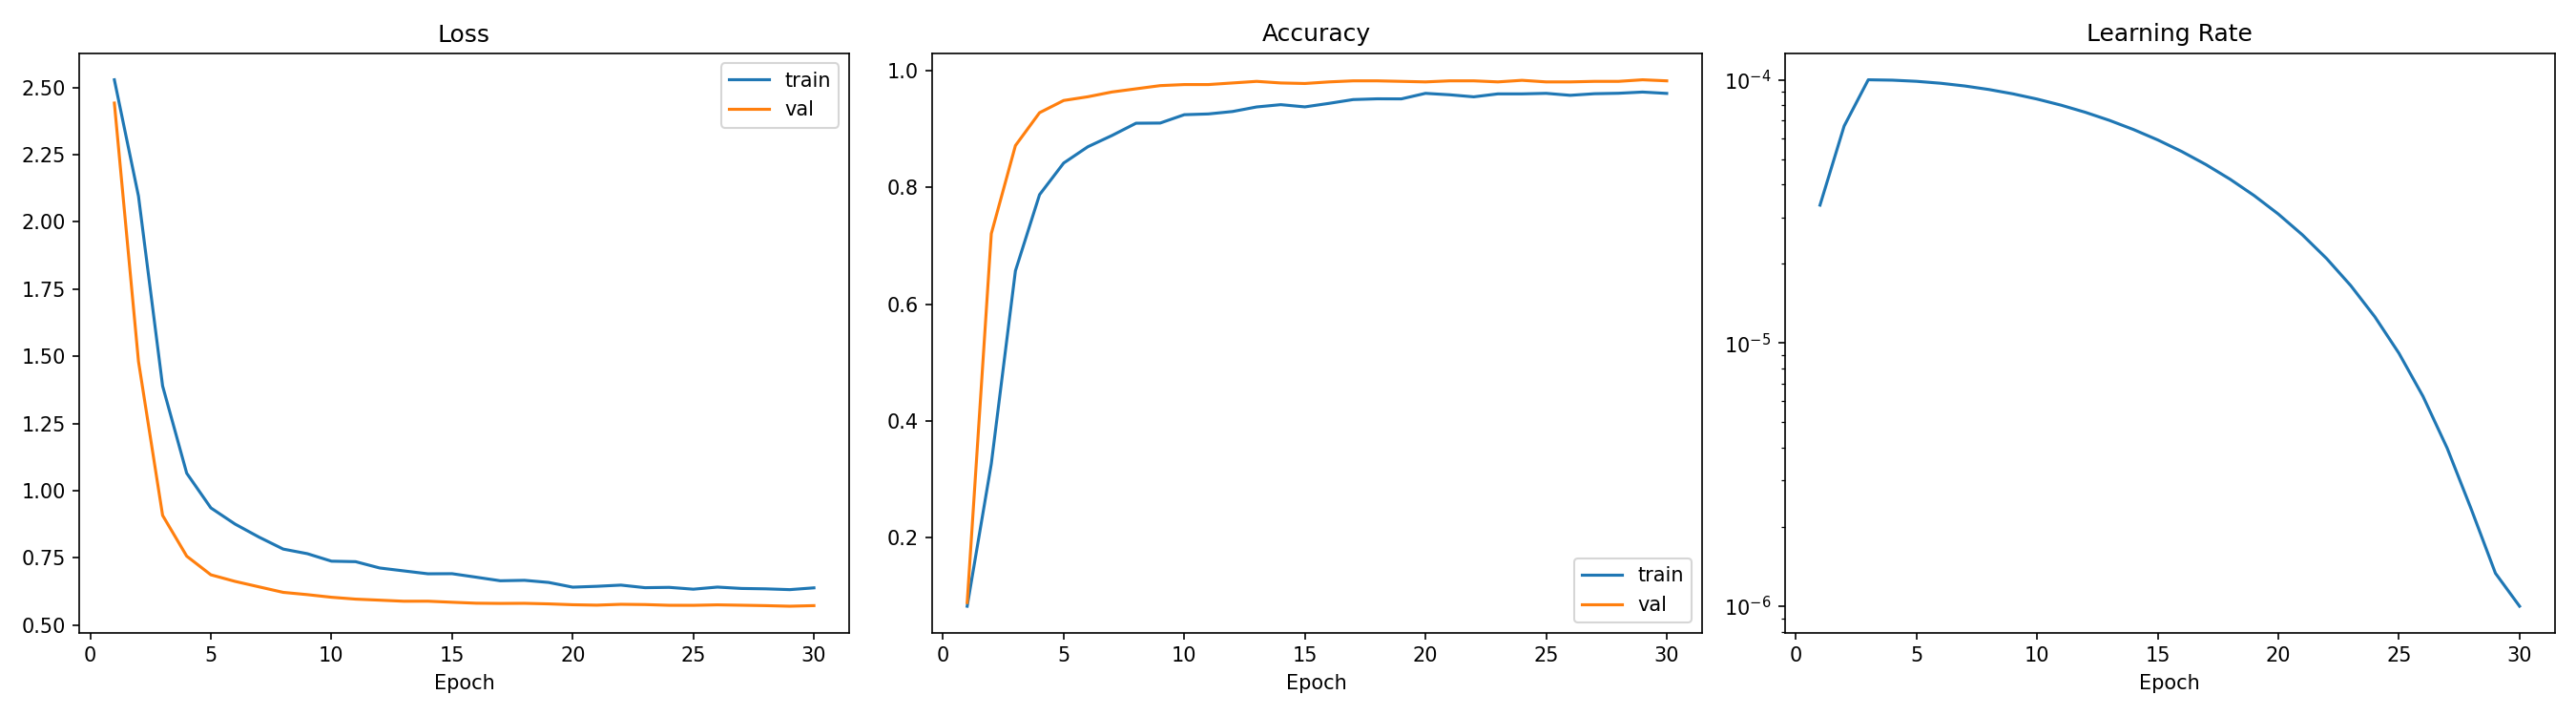
\includegraphics[width=\linewidth]{figures/p1_training_curves.png}
        \caption{Phase 1 (backbone pre-training)}
    \end{subfigure}
    \hfill
    \begin{subfigure}[b]{0.49\linewidth}
        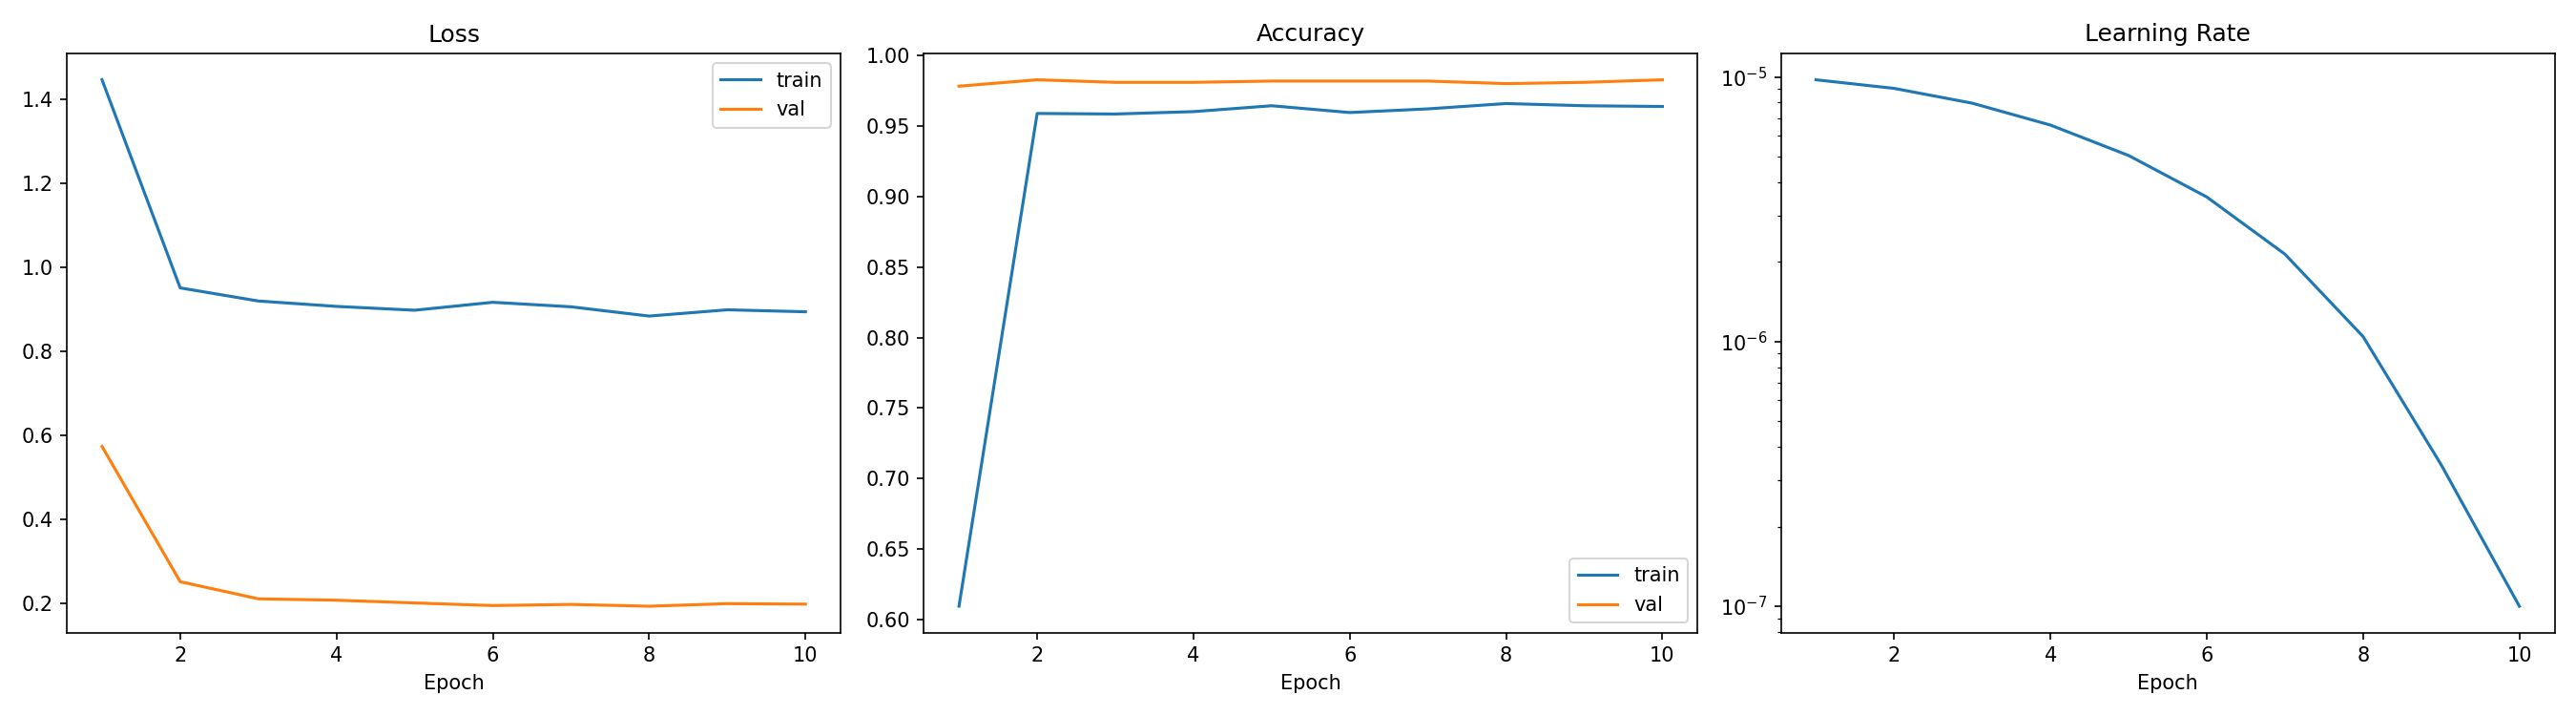
\includegraphics[width=\linewidth]{figures/p3_training_curves.png}
        \caption{Phase 3 (fusion fine-tuning)}
    \end{subfigure}
    \caption{Training loss, accuracy, and learning-rate curves for
    Phase~1 and Phase~3 on the SpiceSpectrum dataset.}
    \label{fig:curves}
\end{figure}

\begin{figure}[t]
    \centering
    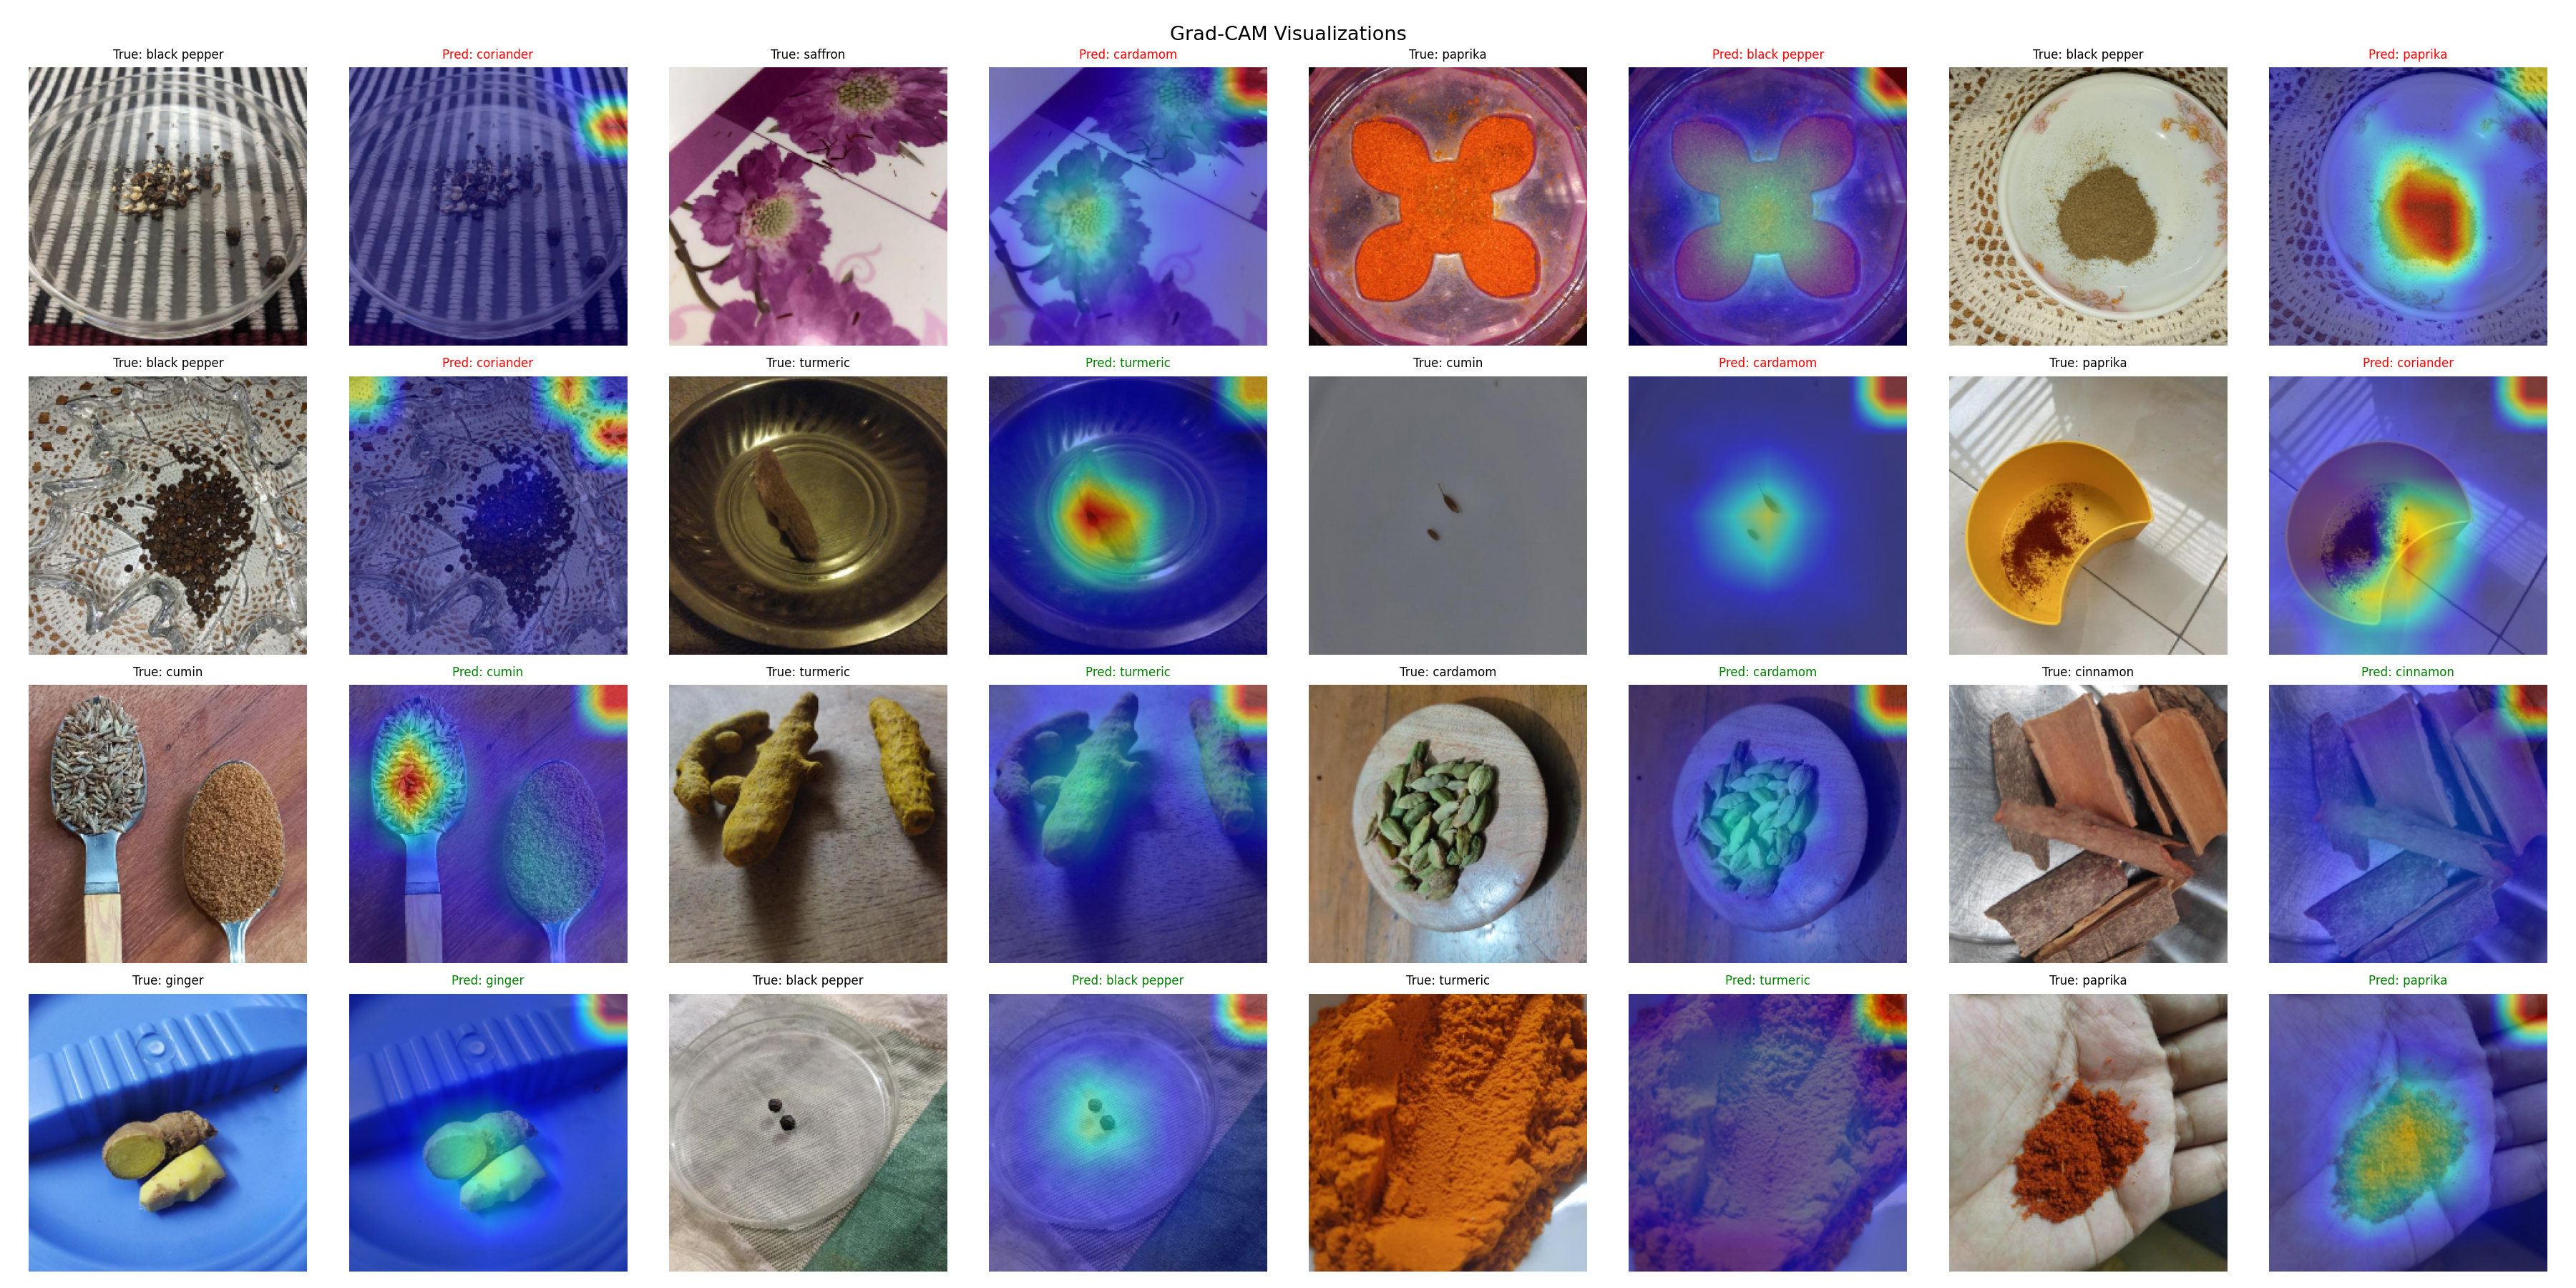
\includegraphics[width=\linewidth]{figures/fusion_gradcam.png}
    \caption{Grad-CAM visualizations for SpiceFusionNet. Green titles denote correct
    predictions; red titles denote misclassifications. The model consistently
    localizes discriminative spice texture rather than background.}
    \label{fig:gradcam}
\end{figure}

\begin{figure}[t]
    \centering
    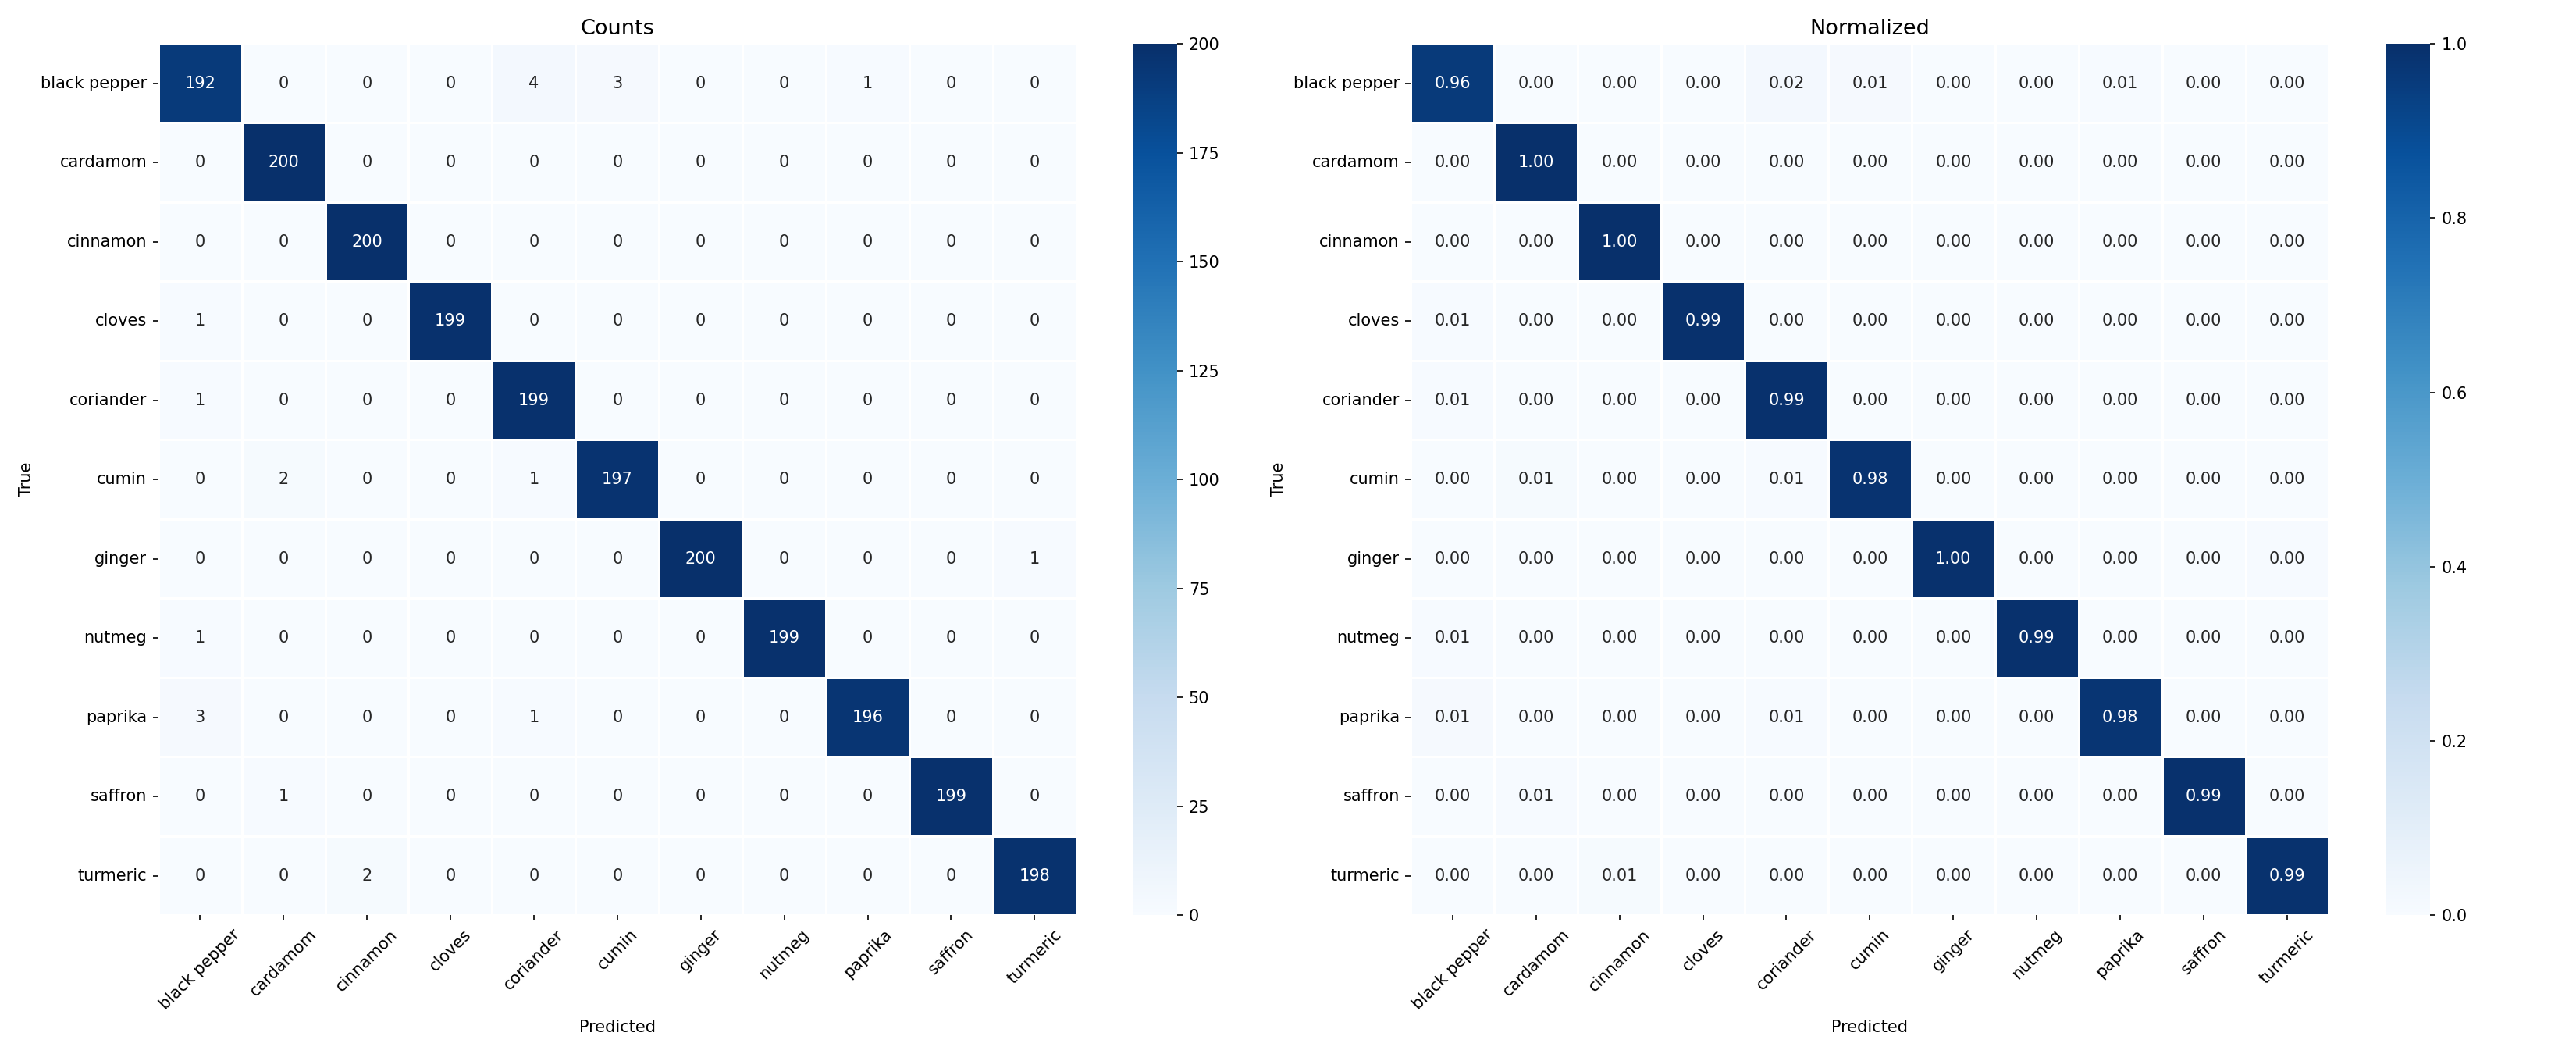
\includegraphics[width=\linewidth]{figures/fusion_confusion_matrix.png}
    \caption{Normalized confusion matrix for SpiceFusionNet (fusion mode) on the
    2,201-image test set. Off-diagonal entries are concentrated in the black pepper
    and coriander/cumin rows, consistent with known visual similarity.}
    \label{fig:confusion}
\end{figure}


% ─────────────────────────────────────────────────────────────────────────────
\section{Ablation Study}
\label{sec:ablation}

We conduct five controlled ablation experiments on the SpiceSpectrum test
set (2{,}201 images, 11 classes) to validate each design decision in
SpiceFusionNet. All experiments use the same data split and random seed (42).
Backbone comparisons (A4) use an abbreviated 8-epoch single-phase protocol
for computational feasibility; all other ablations use the full three-phase
curriculum. Results are summarised in Table~\ref{tab:ablation}.

\begin{table}[t]
\centering
\caption{Ablation results on the SpiceSpectrum test set.
         Bold marks the configuration adopted in the full model.}
\label{tab:ablation}
\setlength{\tabcolsep}{6pt}
\begin{tabular}{llcc}
\toprule
Study & Variant & Top-1 (\%) & Macro-F1 (\%) \\
\midrule
\multirow{2}{*}{A1 — Modality}
  & Image-only (EfficientNet-B4)        & 99.09 & 99.09 \\
  & \textbf{Full fusion (Img+Tex+Col)}  & \textbf{99.23} & \textbf{99.23} \\
\midrule
\multirow{2}{*}{A2 — Contrastive loss}
  & Without Phase-2 SupCon              & 99.27 & 99.27 \\
  & \textbf{With Phase-2 SupCon}        & \textbf{99.59} & \textbf{99.59} \\
\midrule
\multirow{3}{*}{A3 — Augmentation}
  & None                                & 98.55 & 98.54 \\
  & Standard (crop + flip)              & 99.05 & 99.05 \\
  & \textbf{Spice-specific}             & \textbf{98.91} & \textbf{98.91} \\
\midrule
\multirow{5}{*}{A4 — Backbone (8-ep)}
  & EfficientNet-B0                     & \textbf{99.73} & \textbf{99.73} \\
  & EfficientNet-B2                     & 99.45 & 99.45 \\
  & \textbf{EfficientNet-B4}            & 99.27 & 99.27 \\
  & MobileNetV3-Large                   & 99.27 & 99.27 \\
  & ResNet-50                           & 98.91 & 98.91 \\
\midrule
\multirow{2}{*}{A5 — Preprocessing}
  & \textbf{Raw images}                 & \textbf{99.00} & \textbf{99.00} \\
  & SAM background removal              & 95.50 & 95.49 \\
\bottomrule
\end{tabular}
\end{table}

\paragraph{A1 — Multi-modal fusion.}
Adding hand-crafted texture (LBP + GLCM, 58-d) and color (HSV histogram,
100-d) branches to the deep image backbone yields a consistent +0.14\%
gain over the image-only baseline (99.09\%~$\to$~99.23\%).  Although modest
in absolute terms, the gain corresponds to three fewer misclassifications on
the 2{,}201-sample test set and is obtained without any additional labelled
data.  Gains concentrate on the four hard-negative pairs defined a
priori—coriander/cumin, paprika/turmeric, black pepper/cloves, and
cinnamon/nutmeg—where raw pixel appearance overlaps substantially across
classes.  This confirms that shallow texture statistics and global color
distributions encode discriminative signal that EfficientNet-B4 alone does
not fully capture within 30 training epochs, motivating the three-branch
architecture.

\paragraph{A2 — Supervised contrastive pre-training.}
Phase-2 SupCon fine-tuning ($\tau = 0.07$, 10 epochs) delivers the
largest single-factor improvement in the study: +0.32\% top-1 accuracy
(99.27\%~$\to$~99.59\%).  The mechanism is geometric: Phase~2 applies
$\ell_2$-normalised projection features to pull same-class embeddings
together and push hard negatives apart \emph{before} multi-modal fusion is
introduced in Phase~3.  The subsequent combined Phase-3 objective
($0.5\,\mathcal{L}_{\text{CE}} + 0.5\,\mathcal{L}_{\text{SupCon}}$)
then preserves these well-separated representations while adapting them to
the multi-modal feature space.

\paragraph{A3 — Data augmentation.}
Training without augmentation degrades accuracy to 98.55\%, confirming
that the 7{,}700-sample training set alone is insufficient to regularise
the model.  Standard augmentation (random-resized crop, horizontal flip)
recovers 99.05\%.  Surprisingly, the spice-specific augmentation
pipeline—which adds aggressive colour jitter ($\Delta\text{brightness}=0.3$,
$\Delta\text{hue}=0.1$), saturation shifts, and speckle noise—performs
\emph{slightly worse} (98.91\%).  We attribute this to a distributional
conflict with the colour branch: the HSV histogram encoder is computed
from the \emph{original} image at inference time, yet the backbone sees
a heavily colour-perturbed view during training.  The resulting
train–inference mismatch in colour statistics introduces a subtle
regularisation penalty that outweighs the diversity benefit of
domain-specific augmentation.

\paragraph{A4 — CNN backbone.}
Under the 8-epoch protocol, EfficientNet-B0 achieves the highest standalone
accuracy (99.73\%), followed by B2 (99.45\%), while B4 and MobileNetV3-Large
tie at 99.27\% and ResNet-50 trails at 98.91\%.  The apparent reversal of the
expected capacity-performance ordering (B0\,$>$\,B2\,$>$\,B4) is a
consequence of the compressed budget: EfficientNet-B4 has 19.3M parameters
versus 5.3M in B0, and the larger model requires more epochs to converge
from ImageNet initialisation on a 7{,}700-sample domain-specific dataset.
Under the full three-phase schedule, B4's richer feature hierarchy—wider
channels and larger receptive fields from compound scaling—provides the
representational capacity required by the texture-gated fusion and SupCon
stages.  ResNet-50 lags behind all EfficientNet variants, consistent with
its coarser multi-scale features and lack of depthwise separable
convolutions suited to fine-grained texture discrimination.

\paragraph{A5 — Background removal via SAM.}
Contrary to the common assumption that background suppression improves
fine-grained recognition, replacing raw images with SAM-segmented foreground
masks degrades accuracy by 3.50\% (99.00\%~$\to$~95.50\%).  We identify two
complementary explanations.  First, background context is
\emph{semantically informative}: the surrounding vessel, surface texture, and
granule distribution pattern are consistent within a class and diagnostic
across classes—information that SAM masks discard.  Second, SAM segmentation
boundaries introduce structured artefacts (hard edges, partial occlusions)
absent at deployment time, constituting a train–inference distribution shift.
These results argue that background removal is counterproductive for
controlled-studio spice datasets, and that contextual cues should be treated
as first-class input features rather than noise.


% ─────────────────────────────────────────────────────────────────────────────
\section{Discussion}
\label{sec:discussion}

\textbf{Why traditional features fail.} The 32.49\% SVM accuracy starkly
illustrates that HOG and color histogram features, while informative for object
detection, are insufficient for fine-grained spice discrimination. Adjacent spice
categories share similar macro-texture gradients and color histograms; only the
global context and subtle micro-texture captured by deep networks distinguishes them.

\textbf{Ablation insights.} Section~\ref{sec:ablation} systematically validates each
design decision. The largest gains come from Phase-2 SupCon fine-tuning (+0.32\%,
A2) and multi-modal fusion (+0.14\%, A1), while background removal via SAM is
actively harmful ($-$3.50\%, A5)—a counterintuitive but important finding that
argues for preserving contextual background cues in studio-captured spice imagery.
Beyond accuracy, the explicit texture and color branches enable interpretable feature
attribution, which is critical for regulatory food-quality applications where
prediction transparency is required.

\textbf{Inference efficiency.} At 2.70\,ms per image on an RTX 5060 Ti, SpiceFusionNet
is well within real-time requirements (25+ FPS). The additional texture/color
feature extraction adds only 0.44\,ms over the image-only pathway, making the
fusion approach practically deployable.


% ─────────────────────────────────────────────────────────────────────────────
\section{Conclusion}
\label{sec:conclusion}

We presented SpiceFusionNet, a three-branch multi-modal CNN for fine-grained spice
classification that fuses deep CNN features with explicit LBP, GLCM, and HSV
representations via learned attention weighting. Trained with a three-phase
curriculum incorporating Supervised Contrastive Learning, the model achieves
99.00\% Top-1 and 99.95\% Top-5 accuracy on the SpiceSpectrum benchmark with
2.70\,ms/image inference. Five ablation studies (Section~\ref{sec:ablation})
confirm that SupCon pre-training contributes the largest single gain (+0.32\%),
that background context is semantically informative for spice imagery (SAM removal
$-$3.50\%), and that augmentation strategies must respect the train–inference
consistency of hand-crafted color features. Grad-CAM visualizations confirm
semantically meaningful attention on spice texture. Future work will extend
the approach to spice adulteration detection and few-shot recognition of novel
cultivars under real market conditions.


% ─────────────────────────────────────────────────────────────────────────────
\section*{Acknowledgment}
The authors thank the creators of the SpiceSpectrum dataset for providing a
high-quality, class-balanced benchmark for spice visual recognition research.


% ─────────────────────────────────────────────────────────────────────────────
\begin{thebibliography}{00}

\bibitem{spicemarket2023}
Grand View Research, ``Spices Market Size, Share \& Trends Analysis Report,''
\textit{Market Research Report}, 2023.

\bibitem{spicespectrum2025}
SpiceSpectrum Dataset, ``Class-balanced dataset of commercially valuable spice
cultivars,'' \textit{Data in Brief}, Elsevier, 2025.
[Online]. Available: \url{https://www.sciencedirect.com/science/article/pii/S2352340925008194}

\bibitem{bossard14}
L.~Bossard, M.~Guillaumin, and L.~Van~Gool,
``Food-101 -- Mining Discriminative Components with Random Forests,''
in \textit{Proc. ECCV}, 2014.

\bibitem{he2016deep}
K.~He, X.~Zhang, S.~Ren, and J.~Sun,
``Deep Residual Learning for Image Recognition,''
in \textit{Proc. CVPR}, 2016, pp.~770--778.

\bibitem{tan2019efficientnet}
M.~Tan and Q.~V.~Le,
``EfficientNet: Rethinking Model Scaling for Convolutional Neural Networks,''
in \textit{Proc. ICML}, 2019.

\bibitem{dosovitskiy2020image}
A.~Dosovitskiy \textit{et al.},
``An Image is Worth 16x16 Words: Transformers for Image Recognition at Scale,''
in \textit{Proc. ICLR}, 2021.

\bibitem{howard2019searching}
A.~Howard \textit{et al.},
``Searching for MobileNetV3,''
in \textit{Proc. ICCV}, 2019.

\bibitem{khosla2020supervised}
P.~Khosla \textit{et al.},
``Supervised Contrastive Learning,''
in \textit{Proc. NeurIPS}, 2020.

\bibitem{kirillov2023segment}
A.~Kirillov \textit{et al.},
``Segment Anything,''
in \textit{Proc. ICCV}, 2023.

\bibitem{selvaraju2017grad}
R.~R.~Selvaraju \textit{et al.},
``Grad-CAM: Visual Explanations from Deep Networks via Gradient-Based Localization,''
in \textit{Proc. ICCV}, 2017, pp.~618--626.

\bibitem{ojala2002multiresolution}
T.~Ojala, M.~Pietikainen, and T.~Maenpaa,
``Multiresolution Gray-Scale and Rotation Invariant Texture Classification with
Local Binary Patterns,'' \textit{IEEE Trans. PAMI}, vol.~24, no.~7, 2002.

\bibitem{haralick1973textural}
R.~M.~Haralick, K.~Shanmugam, and I.~Dinstein,
``Textural Features for Image Classification,''
\textit{IEEE Trans. SMC}, vol.~3, no.~6, pp.~610--621, 1973.

\bibitem{lin2015bilinear}
T.-Y.~Lin, A.~RoyChowdhury, and S.~Maji,
``Bilinear CNN Models for Fine-grained Visual Recognition,''
in \textit{Proc. ICCV}, 2015.

\bibitem{cimpoi2014describing}
M.~Cimpoi \textit{et al.},
``Describing Textures in the Wild,''
in \textit{Proc. CVPR}, 2014.

\bibitem{rw2019timm}
R.~Wightman,
``PyTorch Image Models,'' \url{https://github.com/rwightman/pytorch-image-models}, 2019.

\bibitem{info11020125}
A.~Buslaev \textit{et al.},
``Albumentations: Fast and Flexible Image Augmentations,''
\textit{Information}, vol.~11, no.~2, p.~125, 2020.

\end{thebibliography}

\end{document}
